
\Opensolutionfile{ans}[ans/ans-2-B1]
\TN
\setcounter{ex}{4}
%%==========Câu 5
\begin{ex}%[2D4C3-2]
	\immini{Một hoa văn trang trí được tạo ra từ một miếng bìa mỏng hình vuông cạnh bằng $10$ cm bằng cách khoét đi bốn phần bằng nhau có hình dạng parabol như hình bên. Biết $AB=5$ cm, $OH=4$ cm. Biết giá trang trí hoa văn $1$ cm$^2$ là $50000$ đồng, tính số tiền cần bỏ ra để trang trí hoa văn đó.
		\choice
		{$2\,553\,333$ đồng}
		{\True $2\,333\,333$ đồng}
		{$2\,780\,333$ đồng}
		{$2\,123\,333$ đồng}
	}{
		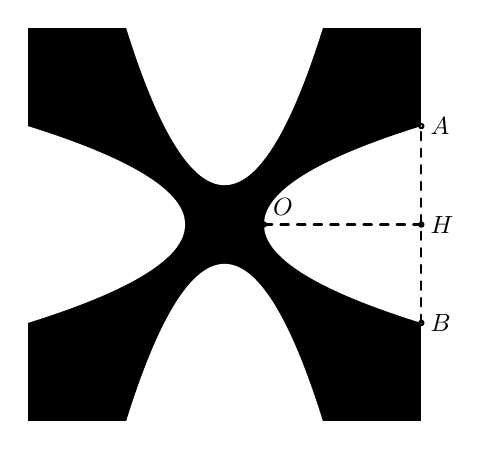
\begin{tikzpicture}[line join=round, line cap=round,>=stealth,thick,scale=0.5]
			\tikzset{every node/.style={scale=0.9}}
			\begin{scope}
				\fill[black] (0,0)--(10,0)--(10,10)--(0,10)--cycle;
				\fill[white](2.5,0)--plot[samples=200,domain=2.5:7.5,smooth,variable=\x] (\x,{-16/25*(\x-2.5)^2+16/5*(\x-2.5)})--(7.5,0);
				\fill[white](2.5,10)--plot[samples=200,domain=2.5:7.5,smooth,variable=\x] (\x,{16/25*(\x-2.5)^2-16/5*(\x-2.5)+10})--(7.5,10);
				\fill[white] plot[samples=200,domain=6:10,smooth,variable=\x] (\x,{sqrt(1.5625*((\x)-6))+5})--(10,5)--plot[samples=200,domain=6:10,smooth,variable=\x] (\x,{-sqrt(1.5625*((\x)-6))+5})--(10,5);
				\fill[white] plot[samples=200,domain=4:0,smooth,variable=\x] (\x,{sqrt(1.5625*(4-(\x)))+5})--(0,5)--plot[samples=200,domain=4:0,smooth,variable=\x] (\x,{-sqrt(1.5625*(4-(\x)))+5})--(0,5);				
			\end{scope}
			\draw[fill=white](6,5) circle (1.5pt) node[above right]{$O$} (10,2.5) circle (1.5pt) node[right]{$B$} (10,7.5) circle (1.5pt) node[right]{$A$} (10,5) circle (1.5pt) node[right]{$H$};
			\draw[dashed] (6,5)--(10,5) (10,2.5)--(10,7.5);
		\end{tikzpicture}
	}
	\loigiai{
		\immini{Đưa parabol vào hệ trục $Oxy$ ta tìm được phương trình là $(P)\colon y=-\dfrac{16}{25}x^2+\dfrac{16}{5}x$.\\
			Diện tích hình phẳng giới hạn bởi $(P)\colon y=-\dfrac{16}{25}x^2+\dfrac{16}{5}x$, trục hoành và các đường thẳng $x=0$, $x=5$ là
			\[S=\displaystyle\int\limits_0^5 \left(-\dfrac{16}{25}x^2+\dfrac{16}{5}x\right)\mathrm{\,d}x=\dfrac{40}{3}.\]
			
		}
		{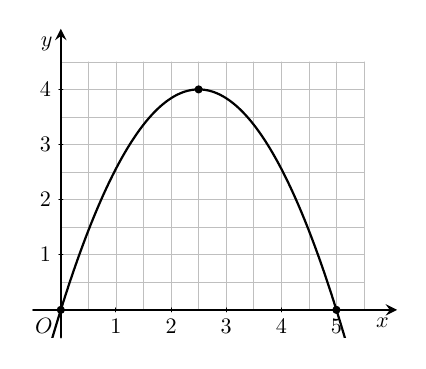
\begin{tikzpicture}[line join=round, line cap=round,>=stealth,thick,scale=0.7]
				\tikzset{every node/.style={scale=0.8}}
				\draw[step=0.5, gray!50,very thin] (0,0) grid (5.5,4.5);
				\draw[->] (-0.5,0)--(6.1,0) node[below left] {$x$};
				\draw[->] (0,-0.5)--(0,5.1) node[below left] {$y$};
				\foreach \x/\nx in {1/1,2/2,3/3,4/4,5/5}
				\draw[thin] (\x,1pt)--(\x,-1pt) node [below] {$\nx$};
				\foreach \y/\ny in {1/1,2/2,3/3,4/4}
				\draw[thin] (1pt,\y)--(-1pt,\y) node [left] {$\ny$};
				\draw (0,0) node [below left] {$O$};
				\begin{scope}
					\clip (-0.5,-0.5) rectangle (5.5,5);
					\draw[samples=200,domain=-0.5:5.5,smooth,variable=\x] plot (\x,{-0.64*(\x)^2+3.2*(\x)+0});
				\end{scope}
				\draw[fill=black](0,0) circle (1.5pt) (2.5,4) circle (1.5pt) (5,0) circle (1.5pt);
			\end{tikzpicture}
		}\noindent
		Tổng diện tích phần bị khoét đi $S_1=4S=\dfrac{160}{3}$ cm$^2$.\\
		Diện tích của hình vuông là $S_{hv}=100$ cm$^2$.\\
		diện tích bề mặt hoa văn là $S_2=S_{hv}-S_1=100-\dfrac{160}{3}=\dfrac{140}{3}\mathrm{\,(cm^2)}$.\\
		Vậy số tiền cần bỏ ra để trang trí hoa văn đó là $\dfrac{140}{3}\cdot 50\,000\approx 2\,333\,333$ (đồng).
	}
\end{ex}
%%==========Câu 6
\begin{ex}%[2D4V3-2]
	\immini{Một viên gạch hoa hình vuông cạnh $40$ cm. Người thiết kế đã sử dụng bốn đường parabol có chung đỉnh tại tâm viên gạch để tạo ra bốn cánh hoa (được tô đen như hình vẽ dưới). Diện tích mỗi cánh hoa của viên gạch bằng
	\choice
	{ $800$ cm$^2$} 
	{ $\dfrac{800}{3}$ cm$^2$} 
	{\True $\dfrac{400}{3}$ cm$^2$} 
	{ $250$ cm$^2$}
	}
	{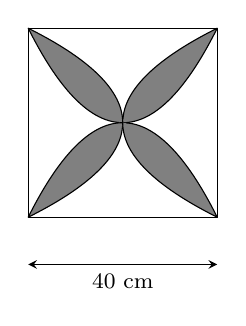
\begin{tikzpicture}[scale=1.2,>=stealth, line join = round, line cap = round,font=\footnotesize]
			\draw (-1,1) rectangle (1,-1);
			\foreach \i in {0,90,180,270}
			\draw [fill=gray, smooth, samples=100,rotate=\i] plot [domain=0:1] (\x, {(\x)^2})-- plot [domain=1:0] (\x, {sqrt(\x)});
			\draw [<-] (-1,-1.5)--(0,-1.5) node[below] {$40$ cm};
			\draw [->] (0,-1.5)--(1,-1.5);
		\end{tikzpicture}
	} 
	\loigiai{
		\immini{Chọn hệ tọa độ như hình vẽ (1 đơn vị trên trục bằng $10$ cm= $1$ dm), các cánh hoa tạo bởi các đường parabol có phương trình $ y=\dfrac{x^2}{2}$, $y=-\dfrac{x^2}{2}$, $x=-\dfrac{y^2}{2}$, $x=\dfrac{y^2}{2}$.\\ 
		Diện tích một cánh hoa (nằm trong góc phàn tư thứ nhất) bằng diện tích hình phẳng giới hạn bởi hai đồ thị hàm số $y=\dfrac{x^2}{2}$, $y=\sqrt{2x}$ và hai đường thẳng $ x=0$; $x=2$.
		}
		{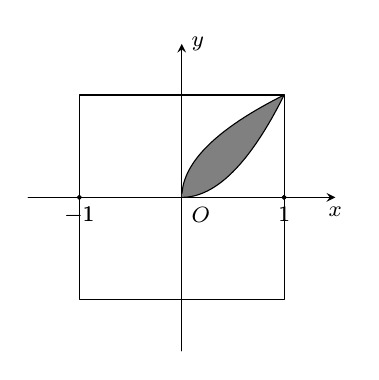
\begin{tikzpicture}[scale=1.3,>=stealth, line join = round, line cap = round,font=\footnotesize]
				\draw[->] (-1.5,0)--(0,0)%
				node[below right]{$O$}--(1.5,0) node[below]{$x$};
				\draw[->] (0,-1.5) --(0,1.5) node[right]{$y$};
				\draw (-1,1) rectangle (1,-1);
				\foreach \i in {-1,1}
				\foreach \j in {-1,1}
				\draw[fill=black]  (\i,0) circle (0.5 pt) node [below] {\footnotesize $\i$};
				\draw [fill=gray, smooth, samples=100] plot [domain=0:1] (\x, {(\x)^2})-- plot [domain=1:0] (\x, {sqrt(\x)});
		\end{tikzpicture}
		}\noindent
	Do đó diện tích một cánh hoa bằng 
	\[\displaystyle\int\limits_0^2 \left( \sqrt{2x}-\dfrac{x^2}{2} \right) \mathrm{d}x = \left(\dfrac{2\sqrt{2}}{3}\sqrt{(2x)^3}-\dfrac{x^3}{6} \right) \Big|_0^2 = \dfrac{4}{3} \;\;\text{dm}^2= \dfrac{400}{3}\;\;\text{cm}^2.\]
	}
\end{ex} 

\chude{Ứng dụng thể tích khối tròn xoay trong bài toán thực tiễn}
\setcounter{ex}{6}
%%==========Câu 7
\begin{ex}%[2D4V3-4]
	\immini{Khi cắt một vật thể hình chiếc niêm bởi mặt phẳng vuông góc với trục $Ox$ tại điểm có hoành độ $x$ ($-2 \le x\le 2$), mặt cắt là tam giác vuông có một góc $45^\circ$ và độ dài một cạnh góc vuông là $\sqrt{14-3x^2}$ (như hình vẽ). Tính thể tích vật thể hình chiếc niêm trên.
	\choice
	{\True $V=20$}
	{$V=20\pi$}
	{$V=10$}
	{$V=10\pi$}
	}
	{\begin{tikzpicture}[declare function={r=4;d=3;},scale=0.6]
			\path (0,0) coordinate (O)--++(85:r/3) coordinate (A)
			($(A)!2!(O)$) coordinate (B)
			($(O)+(0:r)$) coordinate (C)
			($(C)+(90:d)$) coordinate (D)
			;
			\draw (A)..controls +(40:1.5) and +(90:1)..(D)..controls +(-90:1) and +(40:1.5)..(B);
			\draw (A)--(O)node[midway,left]{} (O)--(B)node[midway,left]{} (C)--(D)
			(C)..controls +(-90:1) and +(0:2)..(B)
			;
			\draw[dashed] 
			(A)..controls +(0:2) and +(90:1)..(C)
			(D)--(O) (O)--(C)node[pos=0.7,above]{} ;
			\path pic[draw,angle radius=17pt,"$\alpha$"]{angle= C--O--D};
	\end{tikzpicture}
	}
	\loigiai{
	Diện tích tam giác vuông cân là $S(x)=\dfrac{1}{2}\sqrt{14-3x^2} \cdot \sqrt{14-3x^2} = \dfrac{1}{2}(14-3x^2)$.\\
	Vậy thể tích vật thể là $\displaystyle\int\limits_{-2}^2 \dfrac{1}{2}(14-3x^2)\mathrm{\,d}x=20$.
	}
\end{ex}
%%==========Câu 8
\begin{ex}%[2D4V3-4]
	\immini{Trong chương trình nông thôn mới của tỉnh Phú Yên, tại xã Hòa Mỹ Tây có xây một cây cầu bằng bê tông như hình vẽ (đường cong trong hình vẽ là các đường Parabol). Biết $1$ m$^3$ khối bê tông để đổ cây cầu có giá 5 triệu đồng. Tính số tiền mà tỉnh Phú Yên cần bỏ ra để xây cây cầu trên.
	}
	{\begin{tikzpicture}[scale=1.0, font=\footnotesize, line join=round, line cap=round,>=stealth,samples=100]
			\path 
			(0,0) coordinate (O)
			(-1,0) coordinate (B)
			(0,1) coordinate (C)
			(1,0) coordinate (D)
			(-1.4,0) coordinate (M)
			(0,1.96) coordinate (N)
			(1.4,0) coordinate (P)
			;
			\path (-165:4) coordinate (A);
			\foreach \x in {B,C,D,M,N,P,O}{\path ($(\x)+(-165:4)$) coordinate (\x_1);}
			\fill[gray!40] (N_1)--(N)--plot[domain=0:1.4] (\x,{-(\x)^2+1.96})--(P)--(P_1)--plot[shift={(A)},domain=1.4:0] (\x,{-(\x)^2+1.96});
			\fill[gray!40] (M_1)--plot[shift={(A)},domain=-1.4:1.4](\x,{-(\x)^2+1.96})--(P_1)--(D_1)--plot[shift={(A)},domain=1:-1] (\x,{-(\x)^2+1})--(B_1)--(M_1);
			\draw[dash pattern=on 2pt off 2pt] plot[domain=-1:1] (\x,{-(\x)^2+1})
			plot[domain=-1.4:1.4] (\x,{-(\x)^2+1.96})
			(M)--(P) (O)--(N)
			;
			\draw[shift={(A)}] plot[domain=-1:1] (\x,{-(\x)^2+1});
			\draw[shift={(A)}] plot[domain=-1.4:1.4] (\x,{-(\x)^2+1.96});
			\draw [dash pattern=on 2pt off 2pt] (B)--(B_1) (C)--(C_1) (D)--(D_1) (M)--(M_1)
			(O_1)--(N_1)
			;
			\draw (N)--(N_1) (P)--(P_1) (M_1)--(P_1);
			\foreach \t in {O,B,M,P,O_1,M_1,B_1,D_1,P_1}{
				\draw[fill=white] (\t) circle (1pt);}
			\path (M_1)--(B_1) node[midway,below]{$0,5$m};
			\path (B_1)--(D_1) node[midway,below]{$19$m};
			\path (D_1)--(P_1) node[midway,below]{$0,5$m};
			\path (O)--(C) node[midway,right]{$2$m};
			\path (C)--(N) node[pos=0.2,left]{$0,5$m};
		\end{tikzpicture}
	}
	\choice
	{ $110$ triệu đồng}
	{ $250$ triệu đồng}
	{ $180$ triệu đồng}
	{\True $200$ triệu đồng}
	\loigiai{
		\immini{Chọn hệ trục $Oxy$ như hình vẽ.\\
		Gọi $(P_1)\colon y=a_1 x^2+b_1$ là Parabol đi qua hai điểm $A\left(\dfrac{19}{2};0\right)$, $B(0;2)$.\\
		}
		{\begin{tikzpicture}[scale=0.9, font=\footnotesize, line join=round, line cap=round,>=stealth,samples=100]
				\path 
				(0,0) coordinate (O)
				(-1,0) coordinate (B)
				(0,1) coordinate (C)
				(1,0) coordinate (D)
				(-1.4,0) coordinate (M)
				(0,1.96) coordinate (N)
				(1.4,0) coordinate (P)
				;
				\path (-165:4) coordinate (A);
				\foreach \x in {B,C,D,M,N,P,O}{\path ($(\x)+(-165:4)$) coordinate (\x_1);}
				\fill[gray!40] (N_1)--(N)--plot[domain=0:1.4] (\x,{-(\x)^2+1.96})--(P)--(P_1)--plot[shift={(A)},domain=1.4:0] (\x,{-(\x)^2+1.96});
				\fill[gray!40] (M_1)--plot[shift={(A)},domain=-1.4:1.4](\x,{-(\x)^2+1.96})--(P_1)--(D_1)--plot[shift={(A)},domain=1:-1] (\x,{-(\x)^2+1})--(B_1)--(M_1);
				\draw[-stealth,dash pattern=on 2pt off 2pt] (-1.4,0)--(0,0)node[below left]{$O$}--(2,0) node[below] {$x$};
				\draw[-stealth,dash pattern=on 2pt off 2pt] (0,0)--(0,2.5) node[left] {$y$};
				\draw[dash pattern=on 2pt off 2pt] plot[domain=-1:1] (\x,{-(\x)^2+1})
				plot[domain=-1.4:1.4] (\x,{-(\x)^2+1.96})
				;
				\draw[shift={(A)}] plot[domain=-1:1] (\x,{-(\x)^2+1});
				\draw[shift={(A)}] plot[domain=-1.4:1.4] (\x,{-(\x)^2+1.96});
				\draw [dash pattern=on 2pt off 2pt] (B)--(B_1) (C)--(C_1) (D)--(D_1) (M)--(M_1)
				(O_1)--(N_1)
				;
				\draw (N)--(N_1) (P)--(P_1) (M_1)--(P_1);
				\foreach \t in {O,B,M,P,O_1,M_1,B_1,D_1,P_1}{
					\draw[fill=white] (\t) circle (1pt);}
				\path (M_1)--(B_1) node[midway,below]{$0,5$m};
				\path (B_1)--(D_1) node[midway,below]{$19$m};
				\path (D_1)--(P_1) node[midway,below]{$0,5$m};
				\path (O)--(C) node[midway,right]{$2$m};
				\path (C)--(N) node[pos=0.2,left]{$0,5$m};
			\end{tikzpicture}
		}\noindent
	Nên ta có hệ phương trình sau
	\[\heva{& 0=a\cdot \left(\dfrac{19}{2}\right)^2+2 \\ & 2=b} \Leftrightarrow \heva{& a_1=-\dfrac{8}{361} \\ & b_1=2 }\Rightarrow (P_1)\colon y=-\dfrac{8}{361}{x^2}+2.\]
	Gọi $(P_2)\colon y=a_2 x^2+b_2$ là Parabol đi qua hai điểm $C(10;0)$, $D\left(0;\dfrac{5}{2}\right)$.\\
	Nên ta có hệ phương trình sau
	\[\heva{& 0=a_2 \cdot 10^2 + \dfrac{5}{2} \\ & \dfrac{5}{2}=b_2 } \Leftrightarrow \heva{& a_2=-\dfrac{1}{40} \\ & b_2=\dfrac{5}{2} } \Rightarrow (P_2)\colon y=-\dfrac{1}{40}{x^2}+\dfrac{5}{2}.\]
	Ta có thể tích của bê tông là
	\[V=5\cdot 2\left[\displaystyle\int\limits_0^{10}\left(-\dfrac{1}{40}{x^2}+\dfrac{5}{2} \right)\mathrm{\,d}x-\displaystyle\int\limits_0^{\tfrac{19}{2}}\left( -\dfrac{8}{361}x^2+2\right)\mathrm{\,d}x \right]=40\;\;\text{m}^3.\]
	Số tiền mà tỉnh Phú Yên cần bỏ ra để xây cây cầu là $5\cdot 40=200$ triệu đồng.
	}
\end{ex}
%%==========Câu 9
\begin{ex}%[2D4V3-4]
	Để kỷ niệm ngày 26-3. Chi đoàn 12A dự định dựng một lều trại có dạng parabol, với kích thước: nền trại là một hình chữ nhật có chiều rộng là $3$ mét, chiều sâu là $6$ mét, đỉnh của parabol cách mặt đất là $3$ mét. Hãy tính thể tích phần không gian phía bên trong trại để lớp 12A cử số lượng người tham dự trại cho phù hợp.
	\choice
	{ $30$ m$^3$}
	{\True $36$ m$^3$}
	{ $40$ m$^3$}
	{ $41$ m$^3$}
	\loigiai{
		Giả sử nền trại là hình chữ nhật $ABCD$ có $AB = 3$ m, $BC = 6$ m, đỉnh của parabol là $I$.\\
			Chọn hệ trục tọa độ $Oxy$ sao cho $O$ là trung điểm của cạnh $AB$, $A$, $B$ và $I$, phương trình của parabol có dạng $y=ax^2+b$, $a \ne 0$.\\
			Do $I$, $A$, $B$ thuộc nên ta có $y=-\dfrac{4}{3}x^2+3$.\\
			Vậy thể tích phần không gian phía trong trại là
			\[V=6 \cdot 2\displaystyle\int\limits_0^{\tfrac{3}{2}}\left(-\dfrac{4}{3}x^2+3\right)\mathrm{\,d}x=36.\]
		}
\end{ex}
%%==========Câu 10
\begin{ex}%[2D4V3-4]
	Cho một vật thể bằng gỗ có dạng hình trụ với chiều cao và bán kính đáy cùng bằng $R$. Cắt khối gỗ đó bởi một mặt phẳng đi qua đường kính của một mặt đáy của khối gỗ và tạo với mặt phẳng đáy của khối gỗ một góc $30^\circ$ ta thu được hai khối gỗ có thể tích là $V_1$ và $V_2$, với $V_1<V_2$. Thể tích $V_1$ bằng
	\choice
	{\True $V_1=\dfrac{2\sqrt{3}R^3}{9}$}
	{ $V_1=\dfrac{\sqrt{3}\pi R^3}{27}$}
	{ $V_1=\dfrac{\sqrt{3}\pi R^3}{18}$}
	{ $V_1=\dfrac{\sqrt{3}R^3}{27}$}
	\loigiai{
		\immini{Khi cắt khối gỗ hình trụ ta được một hình nêm có thể tích $V_1$ như hình vẽ.\\
		Chọn hệ trục tọa độ $Oxy$ như hình vẽ.\\
		Nửa đường tròn đường kính $AB$ có phương trình là
		\[y=\sqrt{R^2-x^2}, x \in [-R;R].\]
		}
		{\begin{tikzpicture}[declare function={r=4;d=3;},scale=0.7]
				\path (0,0) coordinate (O)--++(85:r/3) coordinate (A)
				($(A)!2!(O)$) coordinate (B)
				($(O)+(0:r)$) coordinate (C)
				($(C)+(90:d)$) coordinate (D)
				;
				\draw (A)..controls +(40:1.5) and +(90:1)..(D)..controls +(-90:1) and +(40:1.5)..(B);
				\draw (A)--(O)node[midway,left]{$R$} (O)--(B)node[midway,left]{$R$} (C)--(D)
				(C)..controls +(-90:1) and +(0:2)..(B)
				;
				\draw[dashed] 
				(A)..controls +(0:2) and +(90:1)..(C)
				(D)--(O) (O)--(C)node[pos=0.7,above]{$R$} ;
				\path pic[draw,angle radius=17pt,"$\alpha$"]{angle= C--O--D};
		\end{tikzpicture}
		}\noindent
		Một mặt phẳng vuông góc với trục $Ox$ tại điểm $M$ có hoành độ $x$, cắt hình nêm theo thiết diện là $\triangle MNP$ vuông tại $N$ và có $\widehat{PMN}=30^\circ$.\\
		Ta có $NM=y=\sqrt{R^2-x^2} \Rightarrow NP=MN \cdot \tan 30^\circ = \dfrac{\sqrt{R^2-x^2}}{\sqrt{3}}$.\\
		Do $\triangle MNP$ có diện tích $S(x)=\dfrac{1}{2}NM \cdot NP =\dfrac{1}{2}\cdot \dfrac{R^2-x^2}{\sqrt{3}}$.\\
		Thể tích hình nêm là 
		\[V_1=\displaystyle\int\limits_{-R}^R S(x)\mathrm{\,d}x=\dfrac{1}{2}\displaystyle\int\limits_{-R}^R \dfrac{R^2-x^2}{\sqrt{3}}\mathrm{\,d}x=\dfrac{1}{2\sqrt{3}}\left(R^2 x-\dfrac{1}{3}x^3 \right) \Big|_{-R}^R=\dfrac{2\sqrt{3}{R^3}}{9}.\]
		\textbf{Chú ý:} Có thể ghi nhớ công thức tính thể tích hình nêm
		$V_1=\dfrac{2}{3}{R^2}h=\dfrac{2}{3}{R^3}\tan \alpha $, trong đó $R=\dfrac{AB}{2}$, $\alpha =\widehat{PMN}$.
		}
\end{ex}
%%==========Câu 11
\begin{ex}%[2D4V3-4]
	\immini{Cho một mô hình $3-D$ mô phỏng một đường hầm như hình vẽ bên. Biết rằng đường hầm mô hình có chiều dài $5$ cm; khi cắt hình này bởi mặt phẳng vuông góc với đấy của nó, ta được thiết diện là một hình parabol có độ dài đáy gấp đôi chiều cao parabol. Chiều cao của mỗi thiết diện parobol cho bởi công thức $y=3-\dfrac{2}{5}x$ cm, với $x$ cm là khoảng cách tính từ lối vào lớn hơn của đường hầm mô hình. Tính thể tích (theo đơn vị cm$^3$) không gian bên trong đường hầm mô hình (làm tròn kết quả đến hàng đơn vị).
	\choice
	{\True $29$}
	{ $27$}
	{ $31$}
	{ $33$}
	}
	{\begin{tikzpicture}[scale=0.6,declare function={a=0.8;b=0.6;c=0.4;d=0.2;}]
			\tikzset{
				homothety at/.style args={#1 scaled by #2}{shift={($(#1)!#2!(0,0)$)},scale=#2},
			}
			\def\mypath{(-120:2)..controls +(90:0.6) and +(-180:0.6)..(0,3)}
			\def\mydot{(0,3)..controls +(0:0.25) and +(95:0.05)..(60:2)}
			\draw \mypath;
			\draw[dashed] \mydot;
			\path (7,0) coordinate (c1);
			\begin{scope}[homothety at=c1 scaled by a]
				\draw \mypath;
				\draw[dashed] \mydot;
			\end{scope}
			\begin{scope}[homothety at=c1 scaled by b]
				\draw \mypath;
				\draw[dashed] \mydot;
			\end{scope}
			\begin{scope}[homothety at=c1 scaled by c]
				\draw \mypath;
				\draw[dashed] \mydot;
			\end{scope}
			\begin{scope}[homothety at=c1 scaled by d]
				\draw \mypath;
				\draw \mydot;
			\end{scope}
			\path 
			(-120:2) coordinate (A)
			(0,3) coordinate (B)
			(60:2) coordinate (C)
			(0,0) coordinate (O);
			\foreach \x in {A,B,C}{\path ($(c1)!a!(\x)$) coordinate (\x_1);}
			\foreach \x in {A,B,C}{\path ($(c1)!b!(\x)$) coordinate (\x_2);}
			\foreach \x in {A,B,C}{\path ($(c1)!c!(\x)$) coordinate (\x_3);}
			\foreach \x in {A,B,C}{\path ($(c1)!d!(\x)$) coordinate (\x_4);}
			\path ($(A_4)!0.5!(B_4)$) coordinate (D);
			\draw (A)--(A_4) (B)--(B_4) (A_4)--(C_4)
			;
			\draw[dashed] (B)node[above]{$3$}--(O)--(D)node[below right]{$5$} (A)--(C) (A_1)--(C_1) (A_2)--(C_2) (A_3)--(C_3)  (C)--(C_4);
		\end{tikzpicture}
	}
	\loigiai{
		\immini{Xét một thiết diện Parabol có chiều cao là $h$ và độ dài đáy $2h$ và chọn hệ trục $Oxy$ như hình vẽ trên.\\
			Parabol $(P)$ có phương trình $(P)\colon y=ax^2+h$, ($a<0$).\\
			Có $B(h;0)\in (P) \Leftrightarrow 0=ah^2+h \Leftrightarrow a=-\dfrac{1}{h}$ (do $h>0$).\\
			Diện tích $S$ của thiết diện là
			\[S=\displaystyle\int\limits_{-h}^h \left( -\dfrac{1}{h}x^2+h\right)\mathrm{\,d}x=\dfrac{4h^2}{3}, h=3-\dfrac{2}{5}x \Rightarrow S(x)=\dfrac{4}{3}\left(3-\dfrac{2}{5}x\right)^2.\]
		}
		{\begin{tikzpicture}[scale=0.8,font=\footnotesize]
				\path (0,0) coordinate (O)
				(2,0) coordinate (A)
				(0,2) coordinate (B)
				;
				\draw[-stealth] (-3.5,0)--(0,0)--(3,0)node[below]{$x$};
				\draw[-stealth] (0,-1.5)--(0,4)node[left]{$y$};
				\draw[smooth,samples=100] plot[domain=-2:2](\x,{(-1/2)*(\x)^2+2});
				\foreach \x in {O,A,B}{\draw[fill=blue!40] (\x) circle (1pt);}
				\foreach \x in {-3,-2,-1,1}{\draw (\x,0.05)--(\x,-0.05);}
				\foreach \x in {-1,1,3}{\draw (-0.05,\x)--(0.05,\x);}
				\node[above left] at (B) {$h$};
				\path (O)--(A)node[below]{$h$};
				\node at (0,0) [below left]{$O$};
		\end{tikzpicture}
		}\noindent
		Suy ra thể tích không gian bên trong của đường hầm mô hình là
		\[V=\displaystyle\int\limits_0^5 S(x)\mathrm{\,d}x=\displaystyle\int\limits_0^5\dfrac{4}{3}\left(3-\dfrac{2}{5}x\right)^2\mathrm{\,d}x\approx 28{,}888 \Rightarrow V\approx 29\;\;\text{cm}^3.\]
		}
\end{ex}
%%==========Câu 12
\begin{ex}%[2D4V3-3]
	\immini{Chuẩn bị cho đêm hội diễn văn nghệ chào đón năm mới, bạn Minh Hiền đã làm một chiếc mũ “cách điệu” cho ông già Noel có dáng một khối tròn xoay. Mặt cắt qua trục của chiếc mũ như hình vẽ bên dưới. Biết rằng $OO'=5$ cm, $OA=10$ cm, $OB=20$ cm, đường cong $AB$ là một phần của parabol có đỉnh là điểm $A$. Thể tích của chiếc mũ bằng
	\choice
	{$\dfrac{2750\pi}{3}$ cm$^3$}
	{\True $\dfrac{2500\pi}{3}$ cm$^3$}
	{$\dfrac{2050\pi}{3}$ cm$^3$}
	{$\dfrac{2250\pi}{3}$ cm$^3$}
	}
	{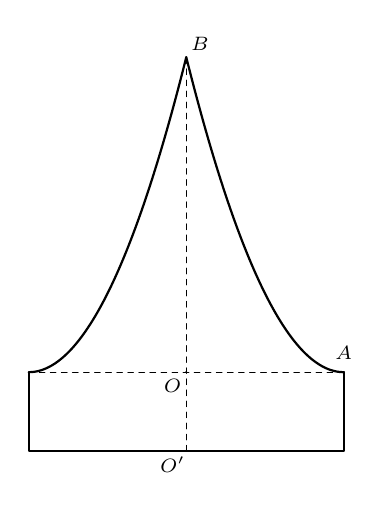
\begin{tikzpicture}[line join=round, line cap=round,>=stealth,scale=0.2]
			\path (0,0) coordinate (O)
			(10,0) coordinate (A)
			(0,20) coordinate (B)
			(0,-5) coordinate (O')
			(10,-5) coordinate (I)
			(-10,-5) coordinate (C)
			(-10,0) coordinate (D)
			;
			\draw[smooth,samples=100,thick] plot[domain=0:10](\x,{(1/5)*((\x)-10)^2})
			plot[domain=-10:0](\x,{(1/5)*((\x)+10)^2})
			;
			\draw[dash pattern=on 2pt off 2pt] (O')--(O)--(B) (A)--(D);
			\draw[thick] (A)--(I)--(C)--(D);
			\foreach \t/\g in {A/90,B/45,O/-135,O'/-135}{
				\draw[fill=black] (\t) circle (1pt) node[shift={(\g:7pt)},font=\scriptsize]{$ \t $};
			}
		\end{tikzpicture}
	}
	\loigiai{
		\immini{Ta gọi thể tích của chiếc mũ là $V$.\\
			Thể tích của khối trụ có bán kính đáy bằng $OA=10$ cm và đường cao $OO'=5$ cm là $V_1$.\\
			Thể tích của vật thể tròn xoay khi quay hình phẳng giới hạn bởi đường cong $AB$ và hai trục tọa độ quanh trục $Oy$ là $V_2$.\\
			Ta có $V=V_1+V_2$; $V_1=5\cdot 10^2\pi =500\pi $ cm$^3$.\\
			Chọn hệ trục tọa độ như hình vẽ.\\
			Do parabol có đỉnh $A$ nên nó có phương trình dạng $(P)\colon y=a(x-10)^2$.
		}
		{\begin{tikzpicture}[line join=round, line cap=round,>=stealth,font=\scriptsize,scale=0.2]
				\path (0,0) coordinate (O)
				(10,0) coordinate (A)
				(0,20) coordinate (B)
				(0,-5) coordinate (O')
				(-10,0) coordinate (C)
				;
				\draw[-stealth] (-12,0)--(0,0)--(12,0)node[below]{$x$};
				\draw[-stealth] (0,-7)--(0,22)node[left]{$y$};
				\draw[smooth,samples=100,thick] plot[domain=0:10](\x,{(1/5)*((\x)-10)^2})
				plot[domain=-10:0](\x,{(1/5)*((\x)+10)^2})
				;
				\draw[thick] (10,0) rectangle (-10,-5);
				\foreach \t/\g in {O/-135,O'/-135}{
					\draw[fill=black] (\t) circle (1pt) node[shift={(\g:7pt)},font=\scriptsize]{$ \t $};
				}
				\draw[fill=black] (A) circle (1pt)node[shift={(45:10pt)}]{$A(10;0)$};
				\draw[fill=black] (B) circle (1pt)node[right]{$B(0;20)$};
				\path (O')--(O)node[pos=0.4,left]{$5$};
				\node at ($(A)+(100:10)$) {$y=\dfrac{1}{5}(x-10)^2$};
			\end{tikzpicture}
		}\noindent
	Vì $(P)$ qua điểm $B(0;20)$ nên $a=\dfrac{1}{5}$.\\
	Do đó, $(P)\colon y=\dfrac{1}{5}(x-10)^2$. Từ đó suy ra $x=10-\sqrt{5y}$ (do $ x<10$).\\
	Suy ra $V_2=\pi \displaystyle\int\limits_0^{20}\left(10-\sqrt{5y}\right)^2\mathrm{\,d}y=\pi(3000-\dfrac{8000}{3})=\dfrac{1000}{3}\pi$ cm$^3$.\\
	Do đó $V=V_1+V_2=\dfrac{1000}{3}\pi +500\pi =\dfrac{2500}{3}\pi$ cm$^3$.
		
	}
\end{ex}
%%==========Câu 13
\begin{ex}%[2D4V3-4]
	\immini{Một chi tiết máy được thiết kế như hình vẽ bên. Các tứ giác $ABCD$, $CDPQ$ là các hình vuông cạnh $2{,}5$ (cm). Tứ giác $ABEF$ là hình chữ nhật có $BE=3{,}5$ (cm). Mặt bên $PQEF$ được mài nhẵn theo đường parabol $(P)$ có đỉnh parabol nằm trên cạnh $ EF$. Thể tích của chi tiết máy bằng
	
	}
	{\begin{tikzpicture}[scale=0.8, font=\footnotesize, line join=round, line cap=round,>=stealth,declare function={a=3;h=4.5;}]
			\path (0,0) coordinate (A)
			--++(30:a) coordinate (B)
			--++(90:a) coordinate (C)
			($(A)+(C)-(B)$) coordinate (D)
			($(A)+(180:h)$) coordinate (F)
			($(B)+(F)-(A)$) coordinate (E)
			($(D)+(180:a)$) coordinate (P)
			($(C)+(P)-(D)$) coordinate (Q)
			;
			\draw (A)--(B)--(C)--(D)--cycle (F)--(A) (D)--(P)--(Q)--(C);
			\draw[dashed] (F)--(E)--(B);
			\draw (F)..controls +(30:1) and +(-100:1)..(P)node[midway,right]{$c$};
			\draw[dashed] (E)..controls +(30:1) and +(-100:1)..(Q)node[pos=0.3,right]{$c$};
			\foreach \t/\g in {A/-90,B/-90,C/0,D/-45,E/135,F/-90,P/180,Q/135}{
				\draw[fill=black] (\t) circle (1pt) node[shift={(\g:7pt)},font=\scriptsize]{$ \t $};
			}
	\end{tikzpicture}
	}
	\choice
	{ $\dfrac{395}{24}$ cm$^3$}
	{ $\dfrac{50}{3}$ cm$^3$}
	{ $\dfrac{125}{8}$ cm$^3$}
	{\True $\dfrac{425}{24}$ cm$^3$}
	\loigiai{
		\immini{Gọi hình chiếu của $P$, $Q$ trên $AF$ và $BE$ là $S$ và $R$.\\
		Vật thể được chia thành hình lập phương $ABCD.PQRS$ có cạnh $2{,}5$ (cm), thể tích $V_1=\dfrac{125}{8}$ cm$^3$ và phần còn lại có thể tích $V_2$.\\
		Khi đó thể tích vật thể $V=V_1+V_2=\dfrac{125}{8}+V_2$.
		}
		{\begin{tikzpicture}[scale=0.7, font=\footnotesize, line join=round, line cap=round,>=stealth,declare function={a=3;h=6;}]
				\path (0,0) coordinate (A)
				--++(30:a) coordinate (B)
				--++(90:a) coordinate (C)
				($(A)+(C)-(B)$) coordinate (D)
				($(A)+(180:h)$) coordinate (F)
				($(B)+(F)-(A)$) coordinate (E)
				($(D)+(180:a)$) coordinate (P)
				($(C)+(P)-(D)$) coordinate (Q)
				($(A)+(P)-(D)$) coordinate (S)
				($(B)+(Q)-(C)$) coordinate (R)
				($(F)!0.5!(S)$) coordinate (M)
				($(M)+(90:2)$) coordinate (M_1)
				($(E)!0.5!(R)$) coordinate (K)
				($(K)+(90:2)$) coordinate (K_1)
				;
				\path[name path=d1] (F)..controls +(30:1) and +(-100:1)..(P);
				\path[name path=d2] (E)..controls +(30:1) and +(-100:1)..(Q);
				\path[name path=d3] (M)--(M_1);
				\path[name path=d4] (K)--(K_1);
				\path[name intersections={of=d1 and d3,by=N}];
				\path[name intersections={of=d2 and d4,by=H}];
				\fill[gray!30] (N)--(M)--(K)--(H)--cycle;
				\draw (A)--(B)--(C)--(D)--cycle (F)--(A) (D)--(P)--(Q)--(C) (P)--(S) (N)--(M);
				\draw[dashed] (F)--(E)--(B) (Q)--(R)--(S) (M)--(K)--(H) (N)--(H);
				\draw (F)..controls +(30:1) and +(-100:1)..(P);
				\draw[dashed] (E)..controls +(30:1) and +(-100:1)..(Q);
				\draw[-stealth] (A)--++(0:1)node[below]{$x$};
				\draw[-stealth] (F)--++(90:1.5*a)node[left]{$y$};
				\foreach \t/\g in {A/-90,B/-90,C/0,D/-45,E/115,F/-90,P/180,Q/135,S/-90,R/-90,N/90,M/-90,K/-90,H/135}{
					\draw[fill=black] (\t) circle (1pt) node[shift={(\g:7pt)},font=\scriptsize]{$ \t $};
				}
			\end{tikzpicture}
		}\noindent
		Đặt hệ trục $Oxyz$ sao cho $O$ trùng với $F$, $Ox$ trùng với $FA$, $Oy$ trùng với tia $Fy$ song song với $AD$. Khi đó Parabol $(P)$ có phương trình dạng $y=ax^2$, đi qua điểm $P\left(1;\dfrac{5}{2}\right)$ do đó $a=\dfrac{5}{2}\Rightarrow y=\dfrac{5}{2}{x^2}$.\\
		Cắt vật thể bởi mặt phẳng vuông góc với $Ox$ và đi qua điểm $M(x;0;0)$, $0\le x\le 1$ ta được thiết diện là hình chữ nhật $MNHK$ có cạnh là $ MN=\dfrac{5}{2}x^2$ và $ MK=\dfrac{5}{2}$ do đó diện tích $S(x)=\dfrac{25}{4}x^2$.\\
		Áp dụng công thức thể tích vật thể ta có $V_2=\displaystyle\int\limits_0^1\dfrac{25}{4}x^2\mathrm{\,d}x=\dfrac{25}{12}$.\\
		Từ đó $V=\dfrac{125}{8}+\dfrac{25}{12}=\dfrac{425}{24}\approx17{,}7$ cm$^3$.

	}
\end{ex}

%%==========Câu 14
\begin{ex}%[2D4V3-4]
	Bổ dọc một quả dưa hấu ta được thiết diện là hình elip có trục lớn $28$ cm, trục nhỏ $25$ cm. Biết cứ $1000$ m$^3$ dưa hấu sẽ làm được cốc sinh tố giá $20000$ đồng. Hỏi từ quả dưa hấu trên có thể thu được bao nhiêu tiền từ việc bán nước sinh tố? Biết rằng bề dày vỏ dưa không đáng kể.
	\choice
	{\True $183000$ đồng} 
	{ $180000$ đồng} 
	{ $185000$ đồng} 
	{ $190000$ đồng}
	\loigiai{ 
		Đường elip có trục lớn $28$ cm, trục nhỏ $25$ cm có phương trình
		\[\dfrac{y^2}{\left(\dfrac{25}{2}\right)^2}=1\Leftrightarrow y^2=\left(\dfrac{25}{2}\right)^2\left(1-\dfrac{x^2}{14^2}\right)\Leftrightarrow y=\pm \dfrac{25}{2}\sqrt{1-\dfrac{x^2}{14^2}}.\]
		Do đó thể tích quả dưa là
		{\allowdisplaybreaks
			\begin{eqnarray*}
				V
				&=& \pi \int\limits_{-14}^{14}\left(\dfrac{25}{2}\sqrt{1-\dfrac{x^2}{14^2}} \right)^2\mathrm{d}x\\
				&=& \pi\left(\dfrac{25}{2}\right)^2\displaystyle\int\limits_{-14}^{14}\left(1-\dfrac{x^2}{14^2}\right)^2\mathrm{d}x\\
				&=&\pi\left(\dfrac{25}{2}\right)^2 \cdot \left(x-\dfrac{x^3}{3\cdot 14^2}\right) \Big|_{-14}^{14}\\
				&=& \pi\left(\dfrac{25}{2}\right)^2 \cdot \dfrac{56}{3}\\
				&=& \dfrac{8750\pi}{3} \;\;\text{cm}^3.
			\end{eqnarray*}
		}
		Do đó tiền bán nước thu được là $\dfrac{8750\pi \cdot 20000}{3\cdot 1000}\approx 183259$ đồng.
	} 
\end{ex} 

\Closesolutionfile{ans}
% \indapan{6}{ans/ans-2-B1}

